\section{Progetto}

Dopo aver analizzato i requisiti presentati nel capitolo 3 si inizia a realizzare il progetto. Si procede come prima cosa con la suddivisione della rete per aree funzionali. La rete deve:
\begin{itemize}
    \item  mantenere elevati standard di sicurezza
    \item  esporre i servizi su internet
\end{itemize}
Queste aree di lavoro vanno tenute separate per soddisfare due dei requisiti indicati dall'azienda: la modularità e la scalabilità.
Per perseguire tale scopo si sceglie di introdurre una seconda macchina virtuale chiamata vm victim che ospiti dei web server e file server. Il nome 'victim' è giustificato dal fatto che ogni possibile attacco in rete sarà direzionato verso questa macchina virtuale, poiché espone dei servizi su internet. Si intende assegnare alla vm firewall ogni responsabilità relativa alla gestione della sicurezza dell'intera rete (firewall e altri strumenti di difesa...), mentre alla vm victim ogni responsabilità circa la gestione di dati e servizi.
Si decide di procedere così:
\begin{itemize}
    \item  Si dedica un intervallo di indirizzi IP 10.50.50.0/24 ad una LAN, chiamata LAN dei server.
    \item  Alla vm firewall viene aggiunta una seconda scheda di rete ens224, con ip 10.50.50.1.
    \item La vm victim appartiene alla LAN dei server, ha un'unica interfaccia ens160 (oltre a quella di loopback) che corrisponde all'indirizzo 10.50.50.3.  Il router di default è 10.50.50.1.
\end{itemize}

In questo modo la vm firewall si trova tra il router e la vm victim. Il router è configurato in modo da rigirare tutto il traffico che proviene da internet sull'interfaccia esterna della vm firewall (ens160). La vm firewall dopo aver filtrato e analizzato i pacchetti li smista tra i vari host della LAN dei server seguendo le regole di forwarding, svolgendo così il ruolo di router per la 10.50.50.0/24. Questa configurazione è perfetta per soddisfare il requisito di modularità e per permettere il corretto funzionamento della rete. Le macchine virtuali sono separate per ruoli, e questo permette di non propagare modifiche e correzioni, bensì qualsiasi intervento ricadrà unicamente nell'aria di competenza.
Una rete realizzata in questo modo è anche scalabile. Se nel prossimo futuro l'azienda decidesse di espandersi e avesse bisogno di creare altre macchine virtuali, potrebbe popolare la LAN dei server con ben altri 252 dispositivi.
Il cuore dell'intera rete è la LAN dei server, su cui vengono installati dei servizi che sono esposti su internet. Per evitare perdita e compromissione dei dati, tentativi di connessione non autorizzati, injection di codice, e altra attività malevola bisogna lavorare sulla vm firewall.

\begin{figure}[htb]
    \begin{center}
        \begin{tabular}{l}
            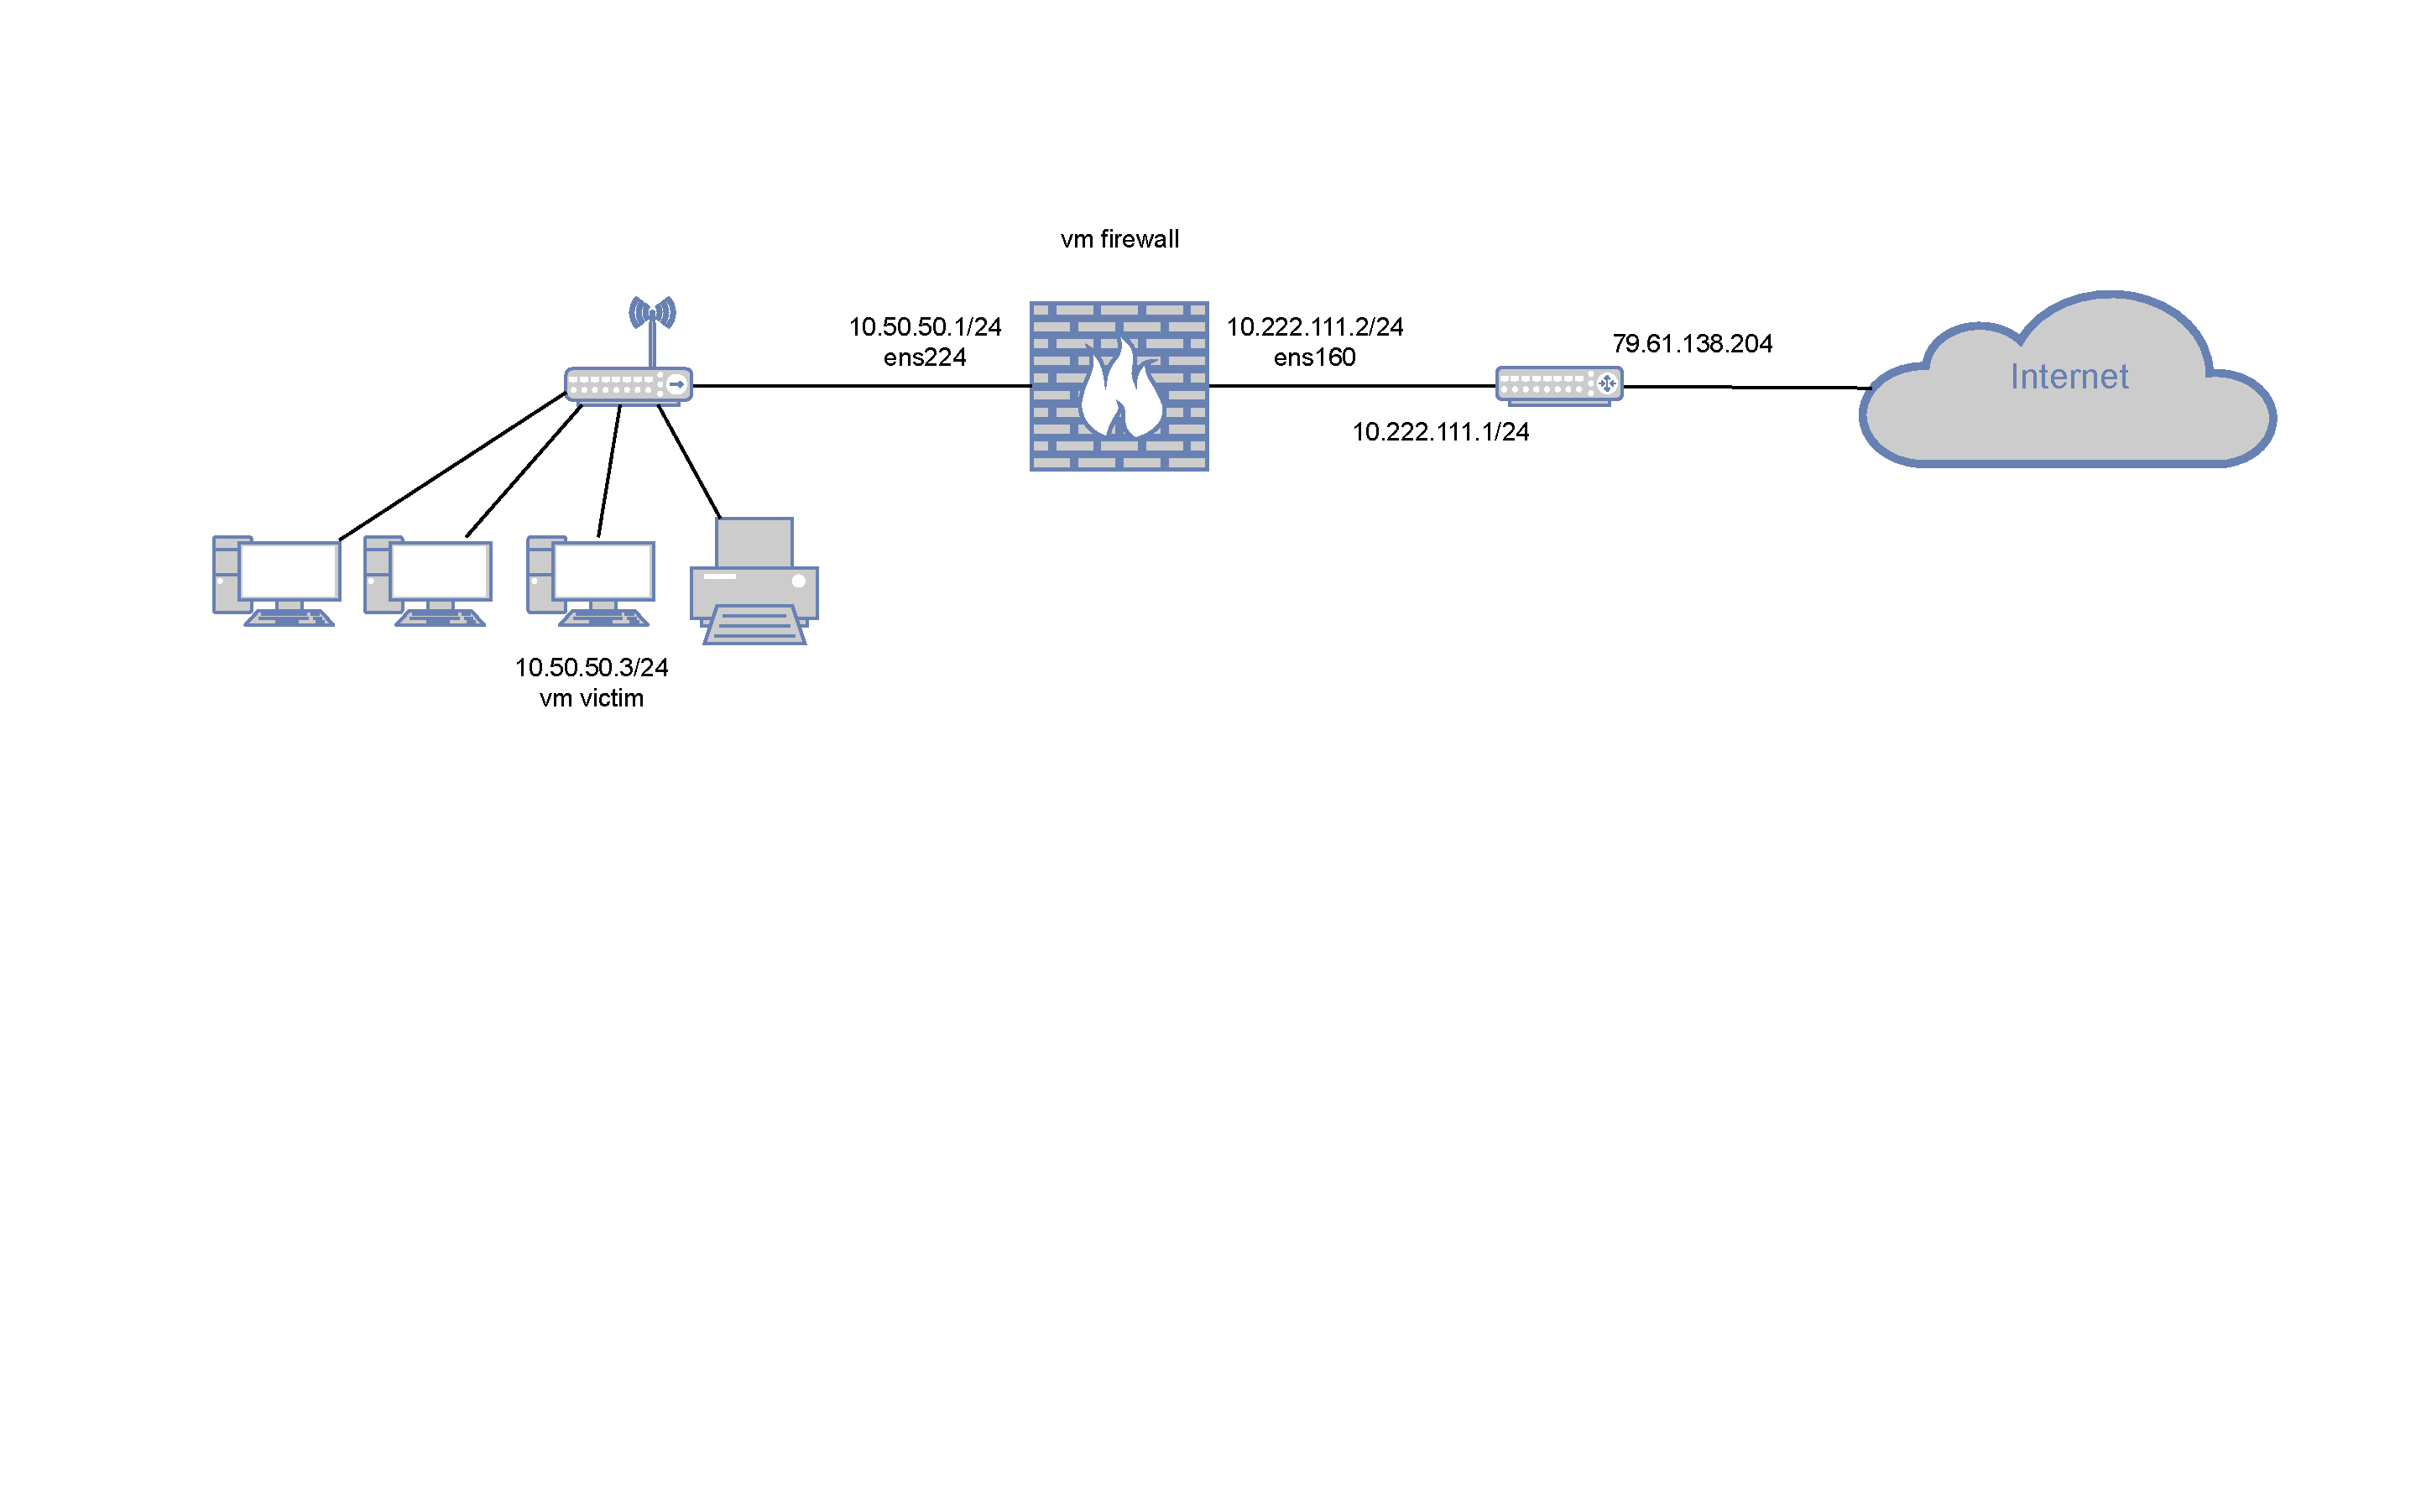
\includegraphics[width=15cm]{figure/net_final.pdf}
        \end{tabular}
    \end{center}
    \caption{Progetto di realizzazione della rete che soddisfi i requisiti imposti nel capitolo 3.}
\end{figure}

Vengono elencati brevemente i vari componenti della rete da sinistra verso destra:

• \textbf{vm victim} nella LAN dei server con una scheda di rete:

– ens160 con IP 10.50.50.3, il router di default è 10.50.50.1

• \textbf{uno switch virtuale}

• \textbf{vm firewall} che ospita il firewall e Snort, con due schede di rete:

– ens160 con IP 10.222.111.2, il router di default è 10.222.111.1

– ens224 con IP 10.50.50.1

• \textbf{il router} con due schede di rete:

– IP privato 10.222.111.1

– IP pubblico 79.61.138.204

Per la realizzazione della macchina virtuale vm victim viene seguita la linea definita dall'azienda e viene utilizzato il sistema operativo CentOS 7.
La macchina viene configurata in questo modo:
\begin{itemize}
    \item  viene settato l'IP statico 10.50.50.3.
    \item  il DNS di riferimento è uno dei DNS server di Google con IP 8.8.8.8.
    \item vengono installati i web server, file server richiesti.
\end{itemize}


Il passo successivo è mostrare nel dettaglio la realizzazione del sistema di rilevazione e prevenzione delle intrusioni con Snort.



